\documentclass[11pt]{article}
\usepackage[margin=1in]{geometry}
\usepackage[T1]{fontenc}
\usepackage{lmodern}
\usepackage{microtype}
\usepackage{graphicx}
\usepackage{booktabs}
\usepackage{tabularx}
\usepackage{amsmath}
\usepackage{xcolor}
\usepackage[numbers,sort&compress]{natbib}
\usepackage[hidelinks]{hyperref}
\usepackage{caption}
\captionsetup{font=small,labelfont=bf}
\setlength{\parskip}{3pt}

\title{Who Writes the System Prompt?\\[2pt]
\large AI Authorship of Frontier-Lab System Prompts as an Outside-In Indicator of AI R\&D Automation}
\author{Hauke Hillebrandt\thanks{Correspondence: \texttt{hauke.hillebrandt@gmail.com}. Draft of 1 October 2026.}}
\date{}

\begin{document}
\maketitle

\begin{abstract}
Frontier AI developers report that AI systems now produce much of their own research and engineering output, but outsiders cannot check these claims. We propose and test an outside-in indicator: the share of newly written text in the system prompts that labs deploy with each model release that is AI-authored. System prompts are public (through official release notes and widely mirrored leaks), dated, rewritten at every release, and written by the labs themselves. We assemble 21 official Anthropic claude.ai prompts (31 dated versions), 15 leaked Anthropic prompt sets and 14 leaked OpenAI prompt sets spanning June 2024 to September 2026, isolate the text that appears for the first time in each version, and score about 220{,}000 words of it with a commercial AI-text detector validated on genre-matched controls, alongside a detector-free stylometric marker. For Anthropic's consumer prompt, the AI-authored share of newly written text averaged 45\% (95\% CI 37--52) through February 2026 and 89\% (81--94) from April 2026, with the best-fitting change point between Claude Opus~4.6 and Opus~4.7. OpenAI's 2025 prompts averaged 23\% (15--31); its 2026 Codex application prompts score 93--95\%. In both labs the shift extends to safety-policy text (Anthropic 46\%$\rightarrow$82\%; OpenAI 29\%$\rightarrow$96\%), and by September 2026 roughly 80--90\% of deployed prompt text was AI-written when first added. AI-authored shares showed no upward drift before the break, and Anthropic's median interval between model releases fell from 73 to 22.5 days. The text that remains human-written is mostly terse interface reference, product facts, legacy passages not yet rewritten and, at OpenAI, agent permission and sandbox rules. We argue that these data strongly support a spring-2026 threshold in the automation of labs' own writing work and independently corroborate their self-reports, but are only weakly informative about recursive self-improvement in the sense of accelerating returns to AI research.
\end{abstract}

\section{Introduction}

Whether automating AI research and development (R\&D) could trigger rapid, self-reinforcing progress is one of the central open questions in AI forecasting and governance \citep{good1966speculations,bostrom2014superintelligence,eth2025sie,chan2026explosion}. A recent multi-author working paper argues that policymakers should ``urgently obtain more visibility into the automation of AI R\&D'', including indicators such as the fraction of research contributions produced by AI systems \citep{chan2026explosion}. The difficulty is that almost all relevant data sit inside the companies. Labs have begun to publish self-reports: Anthropic reports that the AI share of approved code rose from low single digits to over 80\% between January 2025 and May 2026, and that the share of R\&D work completed autonomously rose from 1\% to 26\% between March and August 2026 \citep{favaro2026builds,favaro2026measurements}; OpenAI reports pervasive internal use of code-executing agents \citep{openai2026acceleration}. Outsiders currently have no independent way to check such figures \citep{kwon2026internal,stix2025closed,brundage2026auditing}.

We study one of the few lab-authored documents that is public, versioned and rewritten with every release: the system prompt. Anthropic publishes dated versions of its consumer prompt \citep{anthropic2026sysprompts}, and fuller prompts for both Anthropic and OpenAI products, including tool definitions, are widely mirrored after extraction \citep{cl4r1t4s}. A system prompt is part of the lab's deployment work. Who writes it is a narrow but checkable proxy for how much of the lab's own knowledge work is now done by its models.

Our contributions are:
\begin{enumerate}
\item A measurement design that isolates \emph{first-appearance text}, the text each version adds, so that carried-over passages are not re-counted, and that attributes every sentence of a deployed prompt to the version in which it was written (Section~\ref{sec:methods}).
\item A validated detection pipeline: a commercial detector (Pangram~4) checked against genre-matched human and AI controls, an independent stylometric marker that needs no detector, and a fidelity check of leaked against official text.
\item Evidence from two labs (Section~\ref{sec:results}). Both show a regime shift from roughly a quarter to a half of new prompt text being AI-written to about nine tenths, dated for Anthropic to between February and April 2026, with no upward drift before it. The shift covers safety-policy text.
\item A qualitative analysis of the text that remains human-written in the newest prompts.
\item An assessment of what these data do and do not imply for recursive self-improvement (Section~\ref{sec:discussion}).
\end{enumerate}

\section{Background and related work}
\label{sec:related}

\paragraph{Recursive self-improvement and AI R\&D automation.}
The idea that machines could improve their own successors goes back at least to \citet{good1966speculations} and was developed by \citet{bostrom2014superintelligence}. Recent work formalises a \emph{software intelligence explosion}: if AI systems substitute for researchers, the effective research workforce scales with AI capability, and progress accelerates when returns to research effort exceed diminishing returns ($r>1$) \citep{eth2025sie,ho2025sie,davidson2026feedback,cunningham2026economics,ord2026dynamics}. Empirical estimates draw on the economics of idea production \citep{bloom2020ideas} and algorithmic progress in language models \citep{ho2024algorithmic}, while compute bottlenecks may limit the loop \citep{whitfill2025compute}. Scenario work explores fast transitions \citep{kokotajlo2025ai2027}. \citet{chan2026explosion} synthesise this literature and identify visibility into internal automation as the first policy priority.

\paragraph{Measuring automation of AI R\&D.}
Capability-side measures include task time horizons \citep{kwa2025horizon}, AI R\&D benchmarks such as RE-Bench \citep{wijk2025rebench} and PostTrainBench \citep{rank2026posttrainbench}, and end-to-end automated research pipelines \citep{lu2026endtoend}. \citet{chan2026measuring} propose a taxonomy of indicators of AI R\&D automation, distinguishing capability, usage and outcome measures, and note that usage measures are mostly available only to labs. Labs' own disclosures \citep{favaro2026builds,favaro2026measurements,openai2026acceleration} and third-party reports \citep{metr2026frontier} are the main current sources. Governance work highlights that internal deployment is weakly covered by regulation \citep{kwon2026internal,stix2025closed} and proposes third-party auditing \citep{brundage2026auditing}. Our indicator is a usage measure that outsiders can compute.

\paragraph{Detecting AI-generated text.}
Zero-shot detectors exploit likelihood statistics of a scoring model \citep{mitchell2023detectgpt,bao2024fastdetectgpt,hans2024binoculars}; supervised detectors learn from labelled corpora \citep{verma2024ghostbuster,emi2024pangram}; watermarking embeds a signal at generation time \citep{kirchenbauer2023watermark}. Detection is known to be fragile under paraphrasing \citep{sadasivan2023detect} and biased against some human populations \citep{liang2023bias}. Independent evaluations have found commercial supervised detectors, Pangram in particular, to reach low false-positive rates on long passages \citep{jabarian2025detection}. We use detection at the level of a corpus over time rather than to adjudicate individual authorship, which is the regime where systematic errors partly cancel in comparisons.

\paragraph{Measuring LLM use in the wild.}
A growing literature estimates AI authorship at population scale: in peer reviews \citep{liang2024peer}, scientific papers \citep{liang2024papers}, and biomedical abstracts through excess vocabulary \citep{kobak2025delving}. Stylistic studies characterise the grammatical and rhetorical fingerprints of model prose \citep{reinhart2025pnas}. We apply similar logic to a corpus written by the AI developers themselves.

\paragraph{System prompts and model specifications.}
System prompts sit at the top of an instruction hierarchy that models are trained to respect \citep{wallace2024hierarchy}, and complement training-time specifications such as constitutions and model specs \citep{bai2022cai,anthropic2026constitution,openai2024modelspec}. They can be extracted from deployed models \citep{perez2022ignore,zhang2024extraction}, which is how most of the prompts we study became public. To our knowledge, no prior work has used system prompts as a measurement instrument for lab automation.

\section{Data}
\label{sec:data}

\paragraph{Official Anthropic prompts.} Anthropic's release notes publish the consumer (claude.ai and mobile) system prompt for 21 models, with 31 dated entries from 12 July 2024 to 28 September 2026 \citep{anthropic2026sysprompts}. These exclude tool definitions and product-specific instructions.

\paragraph{Leaked prompts.} The CL4R1T4S repository \citep{cl4r1t4s} mirrors extracted prompts for many products. We use all Anthropic entries (15 prompt sets, June 2024 to September 2026: consumer prompts for each major model, Claude Code, user styles, Claude Design, and a full session capture from Anthropic's agent application) and all OpenAI entries except a 54-word image-generation fragment (14 prompt sets, February 2025 to September 2026: ChatGPT prompts for GPT-4.5, o3/o4-mini, GPT-4o, GPT-4.1 and GPT-5, a personality update, Codex prompts, ChatKit Studio, the Atlas browser, and Codex desktop-application bundles for GPT-5.6 Sol, GPT-6 Astra and GPT-6 Sol). Dates come from the ``current date'' line embedded in each prompt where present, otherwise from the first commit. The Anthropic agent-application file is a full session capture of 272{,}000 words, of which 14\% is system prompt; we use its system prompt, its skill instructions, and a 7{,}200-word sample of its reference files. The 2026 OpenAI files are application-bundle templates with minified identifiers, which suggests direct extraction rather than model recitation.

\paragraph{Fidelity of leaks.} Extraction often works by inducing a model to recite its prompt, which could in principle re-style the text. For Anthropic we compared leaks with official text: all 59 official sentences containing a dash that could be matched in a leak reproduce the original punctuation exactly, including in a leak labelled as a reconstruction. We found no sign that extraction alters the features we measure.

\section{Methods}
\label{sec:methods}

\paragraph{First-appearance text.} Prompts accumulate text across versions, so scoring whole prompts would mostly re-measure old passages. Within each lab we order prompt sets by date and split each into lines (paragraphs, list items, tool-description lines). A line is \emph{new} if at least half of its words lie in sentences never seen in an earlier prompt set of that lab or, for Anthropic, in an official prompt dated strictly earlier. Before matching, model names and dates are normalised and punctuation variants collapsed. For OpenAI, tool descriptions are extracted from JSON by walking all \texttt{description} fields, and code-only lines (e.g.\ TypeScript signatures) are dropped while their comments are kept. This yields 114{,}000 words of new Anthropic prompt text (plus 14{,}000 words of agent-application skill instructions and 158{,}000 words of reference files, of which a 7{,}200-word sample was scored) and 167{,}000 words of new OpenAI text. Because of a fixed detector budget, the two largest OpenAI 2026 files were scored in two rounds: first a systematic sample of contiguous 600-word blocks (31{,}000 words each), then all remaining new text of GPT-5.6 Sol and a further systematic sample of 25{,}000 words of GPT-6 Astra. In total 100\% of GPT-5.6 Sol's and 69\% of GPT-6 Astra's new text was scored; all other new text was scored in full.

\paragraph{Detector.} We use Pangram~4 \citep{emi2024pangram,pangram2026pricing}, which returns document-level AI shares and a segmentation into contiguous passages labelled AI or human with a confidence level. We report the document-level AI share of new text and use the segment labels for section-level and attribution analyses. Segments are mapped back to source lines by aligning each segment's opening characters; all 401 segments were located.

\paragraph{Controls.} We scored genre-matched controls (Figure~\ref{fig:controls}). Anthropic's May 2023 constitution post, written before AI drafting was widespread, scored 0\% AI. Full Claude rewrites of 2024 prompt passages, a 2025 behaviour section and a 2025 tool description scored 91--100\%. A light Claude edit touching about a quarter of the sentences of a human passage scored 43\%. The two earliest official Anthropic prompts, presumed but not known to be human-written, scored 8\% and 14\%. We use these figures for a misclassification sensitivity analysis.

\paragraph{Stylometric marker.} Human authors typing plain text tend to write a dash as a spaced hyphen, whereas Claude models emit the em-dash character. We count em-dashes per 10{,}000 new words in each official Anthropic prompt. The marker needs no detector, but it is model-specific (Section~\ref{sec:results}).

\paragraph{Sections.} Each line is assigned to the innermost enclosing XML tag or heading of its prompt and classified as safety policy (refusals, child safety, wellbeing, copyright, election and harmful-content rules; for agents, approval, sandbox and guardian rules), product and identity, style and behaviour (tone, formatting, personality, final-answer rules), or tools and features. Classification uses keyword rules on section names with a sentence-level fallback (Appendix~\ref{app:sections}).

\paragraph{Stock attribution.} Each sentence inherits the label it received in the prompt set where it first appeared. Summing over a deployed prompt gives the share of that prompt written by AI at the time it was added. Sentences first seen outside the leaks (in official prompts) or in unsampled 2026 OpenAI text are reported as unscored.

\paragraph{Statistics.} Era means are word-weighted across documents, with 95\% confidence intervals from a document-level cluster bootstrap (10{,}000 draws). Change points minimise the word-weighted within-segment sum of squares of a two-mean model. Drift before the break is a word-weighted least-squares slope with bootstrap intervals. For misclassification we invert $p = \mathrm{TPR}\,q + \mathrm{FPR}\,(1-q)$. Release cadence is the gap between successive models' first dated official prompts, compared before and after mid-March 2026 by a one-sided permutation test on medians.

\section{Results}
\label{sec:results}

\begin{figure}[t]
\centering
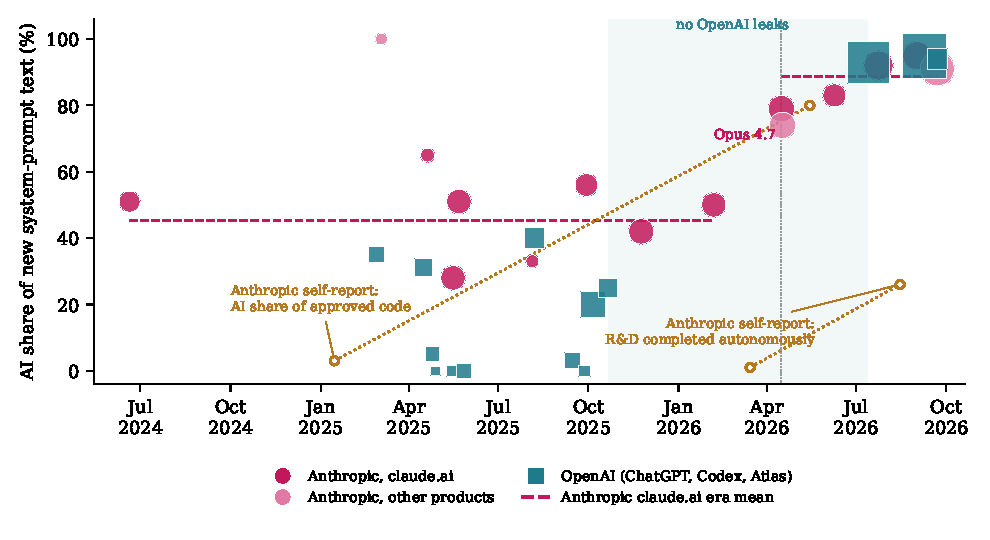
\includegraphics[width=\linewidth]{figs/fig1_new_text.pdf}
\caption{AI-authored share of newly written system-prompt text by release. Marker area is proportional to the amount of new text. Dashed lines are word-weighted era means for Anthropic's consumer prompt. Ringed points are Anthropic's self-reported automation measures \citep{favaro2026builds,favaro2026measurements}, which measure different quantities and are shown for timing only. The shaded interval has no OpenAI observations.}
\label{fig:newtext}
\end{figure}

\paragraph{A regime shift in who writes new prompt text.} Figure~\ref{fig:newtext} shows the AI share of first-appearance text for every prompt set (per-document values in Table~\ref{tab:docs}). For Anthropic's consumer prompt, the word-weighted AI share of new text was 45.2\% (95\% CI 37.0--52.1; 7 releases, 36{,}900 words) from June 2024 to February 2026 and 88.8\% (80.5--93.5; 4 releases, 40{,}500 words) from April to September 2026. Including Anthropic's other products gives 45.9\% and 87.7\%. The best single change point lies between Opus~4.6 (6 February 2026) and Opus~4.7 (16 April 2026). Anthropic's agent-application skill instructions and reference files, first observed in September 2026, score 100\% and 99\%. For OpenAI, new text in 2025 averaged 23.0\% (14.6--31.0; 11 prompt sets), with ChatGPT prompts at 0--40\% and Codex prompts at 0--3\%. The three 2026 Codex-application prompt sets score 93\%, 95\% and 94\% (word-weighted 94.1\%, CI 93.0--95.0). OpenAI has no observations between October 2025 and July 2026, so its change can only be dated to that window, which contains Anthropic's.

\paragraph{No drift before the break.} Before the break, the AI share of new Anthropic text showed no detectable trend ($+1.5$ percentage points per year, 95\% CI $-11.9$ to $+33.9$), and the same holds for OpenAI in 2025 ($-9.2$, CI $-56.7$ to $+45.3$). AI-assisted drafting was present throughout 2024--2025 at a roughly stable level and then stepped up.

\begin{figure}[t]
\centering
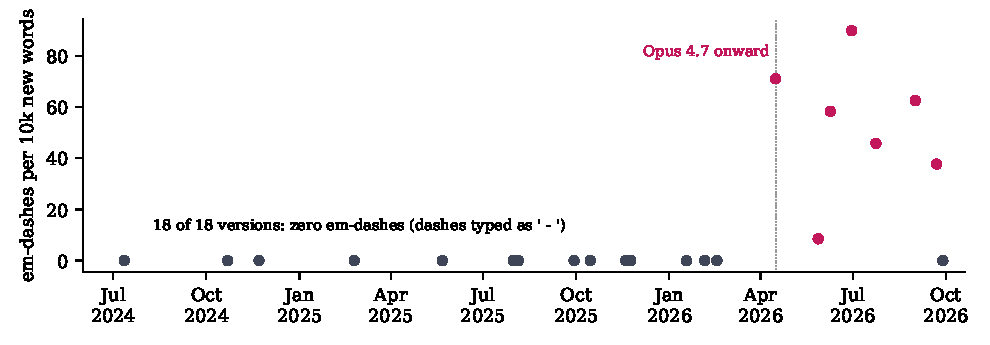
\includegraphics[width=\linewidth]{figs/fig4_emdash.pdf}
\caption{Detector-free check on Anthropic's official consumer prompts: em-dashes per 10{,}000 newly added words in each dated version with at least 50 new words.}
\label{fig:emdash}
\end{figure}

\paragraph{An independent stylometric confirmation.} In every one of the 18 official Anthropic versions published before April 2026 with at least 50 new words, the new text contains no em-dashes; dashes are typed as spaced hyphens. From Opus~4.7 onwards, seven of eight versions contain 8.5--90 em-dashes per 10{,}000 new words (Figure~\ref{fig:emdash}). This marker dates the shift to the same release as the detector, with no detector involved. It does not transfer to OpenAI, whose 2026 Codex-application prompts contain only 4--10 em-dashes per 10{,}000 words although the detector scores them 94\% AI, consistent with OpenAI models emitting fewer em-dashes. In Anthropic's agent-application skill instructions only 59\% of dashes are em-dashes (about 90\% elsewhere in 2026 text), and spaced hyphens appear inside sentences that otherwise read as model prose. This is consistent with partial scrubbing and shows how easily a single stylistic marker can be defeated.

\begin{figure}[t]
\centering
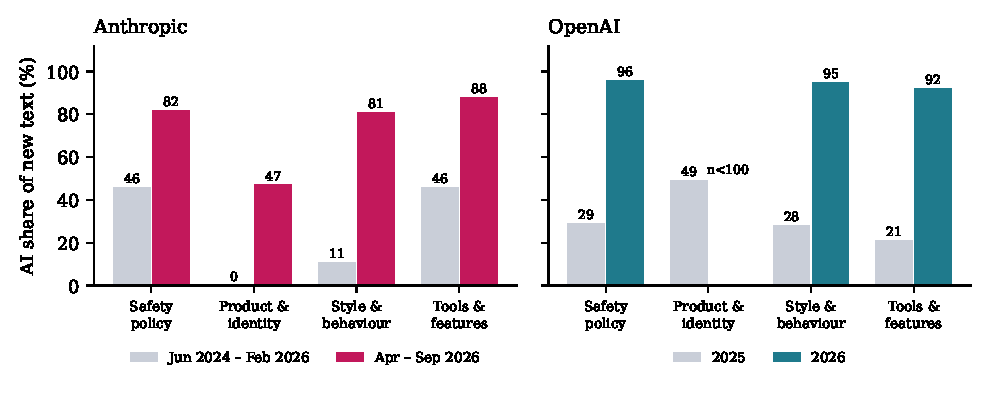
\includegraphics[width=\linewidth]{figs/fig3_sections.pdf}
\caption{AI-authored share of new text by prompt section, before and after the regime shift. Numbers above bars are percentages; cells with fewer than 100 words are marked.}
\label{fig:sections}
\end{figure}

\paragraph{What was delegated.} Before the shift, AI-authored text at Anthropic was concentrated in tool and feature documentation (46\%) and in copyright and search rules, while text describing the model's character and product identity was almost entirely human-written (style 11\%, product 0\%). OpenAI's 2025 shares were lower and similar across sections (21--29\% in every section with at least 500 words). After the shift the distinction disappears (Figure~\ref{fig:sections}): safety-policy text is 82\% AI-authored at Anthropic (from 46\%) and 96\% at OpenAI (from 29\%), and style and behaviour text is 81\% and 95\%.

\begin{figure}[t]
\centering
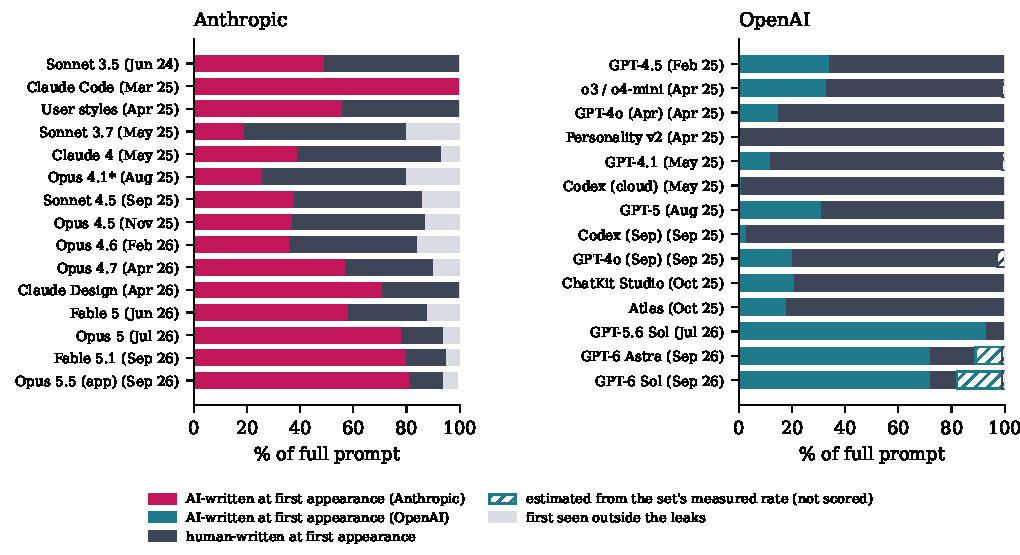
\includegraphics[width=\linewidth]{figs/fig2_stock.pdf}
\caption{Authorship of each deployed prompt. Every sentence carries the label it received in the prompt set where it first appeared. Light grey: text first seen outside the leaks (Anthropic official prompts). Hatched: text never sent to the detector, apportioned at the measured AI rate of the prompt set where it first appeared.}
\label{fig:stock}
\end{figure}

\paragraph{Most deployed prompt text is now AI-written.} Attributing each sentence to its first appearance (Figure~\ref{fig:stock}), Anthropic's consumer prompts were 19--39\% AI-written and 48--61\% human-written through early 2026. By Opus~5.5 (September 2026) the shares are 81\% and 13\%: older human sections were rewritten as well as extended. OpenAI's 2025 prompts were 0--34\% AI-written; its 2026 Codex-application prompts are 82--93\% AI-written and 7--18\% human-written, where 0--18\% of each prompt (text never sent to the detector) is apportioned at the measured rate of the prompt set in which it first appeared.

\paragraph{What is still written by humans.} We read every passage labelled human in the newest prompt sets (Anthropic Opus~5, Fable~5.1 and Opus~5.5; OpenAI GPT-5.6 Sol, GPT-6 Astra and GPT-6 Sol): 5{,}100 and 9{,}600 words of new text respectively, plus carried-over text that was human-written when first added. Table~\ref{tab:qual} summarises the themes. Four observations stand out. First, much of the remaining human text is terse interface reference that is tightly coupled to code, such as parameter descriptions (``The absolute path to the file to modify'', ``Start X coordinate'') and chart-axis options. Such short fragments are also where detectors are least reliable, so part of this category may be undetectable rather than human-written. Second, human authorship persists where facts must be exact: product names and surfaces, documentation URLs, network allow-lists and administrative settings. Third, a substantial share is legacy text that has survived rewriting. OpenAI's \texttt{AGENTS.md} specification first appears in the May 2025 Codex prompt and is carried verbatim into GPT-6, where it is the most repeated human-labelled block, and Anthropic's Opus~5.5 prompt retains human-written self-harm, child-safety and even-handedness rules introduced between November 2025 and June 2026. Fourth, at OpenAI the largest group of newly written human text is operational safety for agents: Windows rules against composing destructive filesystem commands across shells, criteria for requesting escalation outside the sandbox, reviewer instructions for a coding sub-agent's network access, and descriptions of private model-only memory tools (``Never disclose results or this activity''). At Anthropic the clearest newly written human passages are a reflective policy passage on memory and overfamiliarity, written in an idiosyncratic personal voice (``There are some important disanalogies in human <-> human and AI <-> human relations''), and a section on conversational register. Human-labelled passages also contain the only typos and non-native constructions we found (``explicity uses'', ``suggested modifictions'', ``this can be use for'', ``parallelism resolve the task faster''), which corroborates the detector's labels. The overall pattern is that normative and stylistic guidance has been delegated to models, while humans still write text that must match code or facts exactly and some of the rules that constrain agents' actions.

\begin{table}[t]
\centering
\small
\caption{Themes in human-labelled text in the newest prompt sets (qualitative coding; approximate shares of human-labelled new words from keyword-assisted coding).}
\label{tab:qual}
\begin{tabularx}{\linewidth}{>{\raggedright\arraybackslash}p{3.3cm}>{\raggedright\arraybackslash}p{2.3cm}X}
\toprule
Theme & Share (Anthropic / OpenAI) & Examples \\
\midrule
Terse interface and parameter reference & 27\% / 23\% & File-editing and search tool parameters; chart axis options; computer-use coordinates and key syntax \\
Examples, templates, placeholders & 28\% / 28\% & Example user requests; JSON payloads for task and web tools; placeholder lessons in a memory template \\
Agent safety, permission and sandbox rules & 16\% / 29\% & Windows destructive-command rules; escalation criteria; sub-agent network review; hidden memory-tool disclosure rules; targeting of private individuals \\
Product facts, names, URLs, settings & 18\% / 1\% & Product and surface lists; documentation URLs; network allow-lists; admin settings \\
Engineering process documentation & -- / 13\% & Skill-creation guide; code-review guidelines; context-compaction prompt; multi-agent orchestration \\
Policy prose in a distinctive voice & 5\% / -- & Memory and overfamiliarity passage; conversational-register guidance \\
\midrule
Legacy human text carried forward & \multicolumn{2}{p{0.62\linewidth}}{OpenAI: \texttt{AGENTS.md} spec (May 2025), image-generation rules (Apr 2025), web-tool lines (Apr 2025). Anthropic: self-harm rules (Nov 2025), child-safety lines (Apr 2026), political even-handedness (Jun 2026), places, weather and sports tool text.} \\
\bottomrule
\end{tabularx}
\end{table}

\begin{figure}[t]
\centering
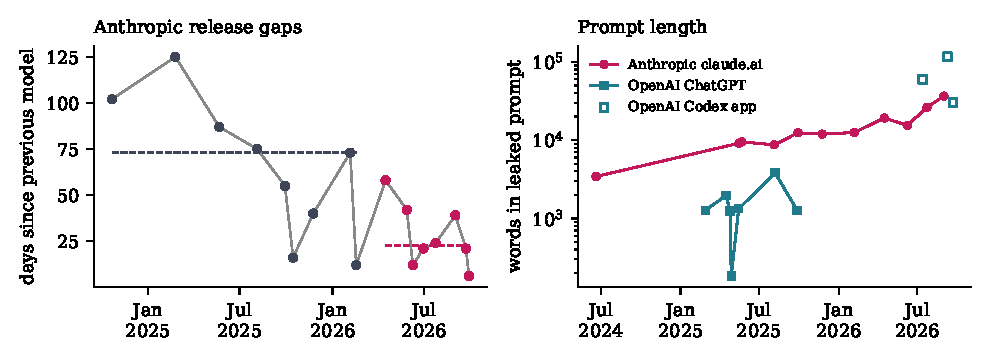
\includegraphics[width=\linewidth]{figs/fig5_cadence.pdf}
\caption{Left: days between successive Anthropic model releases (first dated official prompt), with medians before and after mid-March 2026. Right: length of leaked prompts (log scale).}
\label{fig:cadence}
\end{figure}

\paragraph{Volume and cadence.} Anthropic's median gap between new models fell from 73 days (9 gaps, October 2024 to February 2026) to 22.5 days (8 gaps, April to September 2026; one-sided permutation $p=0.011$). Prompt length grew from 3{,}400 words (June 2024) to about 8{,}700--12{,}500 (2025) and 15{,}000--36{,}000 (2026) for Anthropic's consumer prompt, and from 1{,}200--4{,}800 words (2025 ChatGPT) to 30{,}000--116{,}000 (2026 Codex application) for OpenAI (Figure~\ref{fig:cadence}). Words newly added to Anthropic's official core prompt, however, stayed at about 1{,}000--2{,}000 in most quarters (4{,}100 in the fourth quarter of 2024), with about 6{,}000 in the second quarter of 2026; most of the growth is new products and tools.

\paragraph{Robustness.} Correcting for misclassification with a false-positive rate of 0 (the 2023 human control) and a true-positive rate of 0.97 (the mean of the AI controls) gives Anthropic 47\%$\rightarrow$92\% and OpenAI 24\%$\rightarrow$97\%. Using the 2024 official prompts' 11\% as an upper-bound false-positive rate gives 40\%$\rightarrow$90\% and 14\%$\rightarrow$97\%. The before--after contrast is therefore not an artefact of plausible detector error. The sampling of the two largest OpenAI files is also validated: the unsampled half of GPT-5.6 Sol, scored in the second round, is 92\% AI-authored against 94\% in the first-round sample, and the second GPT-6 Astra sample scores 97\% against 94\%. Because light AI editing registers only partly (43\% for our edited control), the pre-2026 shares are best read as a mixture of AI-drafted and AI-polished text, and the post-shift shares as near-complete AI drafting.

\section{Discussion: what this implies for recursive self-improvement}
\label{sec:discussion}

The intelligence-explosion mechanism has two parts: AI systems expand the effective R\&D workforce as they take over tasks, and that workforce produces better systems that expand it further \citep{chan2026explosion}. Our data bear on the first part, in one small domain.

\paragraph{Evidence consistent with the mechanism.} First, the shift is a threshold rather than gradual adoption: about two years at a stable 25--50\%, then a step to about 90\% within two months of a model generation. This is what one expects if a task becomes automatable once models cross a capability level, the pattern by which automation is expected to spread through the R\&D pipeline. Second, the timing matches Anthropic's self-reports of automation \citep{favaro2026builds,favaro2026measurements}, so the indicator provides independent outside corroboration of claims that otherwise rest on trust. Third, the automation extends to the text that governs model behaviour, including safety policy, which is a concrete instance of humans shifting from authors to reviewers, the oversight risk flagged by \citet{chan2026explosion}. Fourth, rewriting became cheap: most human-written prompt text was replaced within five months, and release intervals shortened by about two-thirds.

\paragraph{Evidence against, and limits.} First, there is no sign of compounding before 2026: AI assistance was substantial for about two years without the share rising. One step does not establish a feedback loop; an explosion would require subsequent steps to arrive faster. Second, system prompts are deployment configuration. Their authorship carries no information about returns to research effort, compute bottlenecks or capability growth rates, which determine whether progress accelerates \citep{eth2025sie,whitfill2025compute,ho2025sie}. Third, AI-written does not mean AI-decided: people may specify and approve every line, and the residual human text shows that humans still author exact facts, code-coupled interface text and some agent safety constraints. Fourth, release cadence has other causes, including product tiering, point releases and competition, and the volume of new core-prompt text did not rise steadily.

\paragraph{Net assessment.} In likelihood terms, the observations are far more probable if labs' internal knowledge work crossed an automation threshold in early 2026 than if it did not, and they are only modestly more probable under a software intelligence explosion than under rapid automation without explosive dynamics. They should therefore raise confidence substantially in the first proposition and only slightly in the second. The most informative next observation is whether the interval to the next comparable step shortens.

\paragraph{Implications for measurement and governance.} The indicator is cheap (about US\$120 of detector credits at list API prices for this study), reproducible, and available to any third party, which makes it a candidate for routine monitoring alongside lab disclosures \citep{chan2026measuring,brundage2026auditing}. It is also easy to game: Anthropic's own prompts include lists of ``Claude-isms'' for its models to avoid, some of the text we analysed appears to have been scrubbed of em-dashes, and detectors can be evaded by paraphrasing \citep{sadasivan2023detect}. It would be more robust if labs disclosed authorship and review processes for system prompts, and in particular for safety-policy text, as part of reporting on internal deployment \citep{kwon2026internal,stix2025closed}.

\section{Limitations}

Detector labels are probabilistic, calibrated here on a small number of controls, and lack a human-written control in the technical-documentation genre, so early tool-documentation shares may include false positives. The leaked corpus is an opportunistic sample: product surfaces differ across time (consumer chat, coding agents, design and agent applications), some releases have no leak, and the 2026 OpenAI data come only from Codex-application bundles. Two large OpenAI files were sampled. Section classification uses keyword heuristics. Dates come from embedded date lines or commit dates and may lag internal authorship. Finally, the indicator measures one kind of writing in two labs and should not be generalised to research work as a whole.

\section{Ethics statement}

All prompts analysed were already public, either published by Anthropic or mirrored in a public repository after extraction by third parties. We performed no extraction and did not interact with any model to obtain prompts. We report aggregate authorship statistics and short identifying fragments only. Detector judgements about individual passages are probabilistic and should not be used to attribute authorship to identifiable individuals.

\section{Conclusion}

Who writes a lab's system prompts is a narrow but public window onto how much of its own work its models do. Across two frontier developers the answer changed in 2026: from roughly a quarter to a half of newly written prompt text to about nine tenths, including the rules that govern model safety. This corroborates labs' accounts of rapid internal automation. Whether that automation is self-accelerating is a different question, which this window can only partly illuminate. Repeating the measurement at future releases will show whether the next step comes sooner.

\section*{Disclosure of AI assistance}
The analysis pipeline (data collection scripts, detector submission, statistics and figures) and a first draft of this paper were produced with substantial assistance from Claude Opus~5.5 (Anthropic), working under the author's direction; the AI-authored control texts were written by the same model. Because the assistant is an Anthropic model and Anthropic is one of the two developers studied, readers should weigh this potential conflict. The author takes full responsibility for the content.

\section*{Data and code availability}
Scripts, the first-appearance texts submitted to the detector, segment-level labels and all derived results are available from the author [repository link to be added].

\bibliographystyle{plainnat}
\bibliography{refs}

\appendix
\section{Per-document results}
\label{app:docs}
\begin{table}[h]
\centering
\scriptsize
\caption{First-appearance text and detector results for every prompt set. ``Scored'' differs from ``new'' only for the two sampled OpenAI files. ``Stock'' gives the AI / human shares of the full deployed prompt by first-appearance attribution (OpenAI 2026 includes text apportioned at measured rates). *Opus~4.1 is a model reconstruction.}
\label{tab:docs}
\resizebox{\textwidth}{!}{%
\begin{tabular}{llllrrrr}
\toprule
Lab & Prompt set & Date & Surface & New words & Scored & AI\% (new) & Stock AI/human\% \\
\midrule
%% rows generated by make_tables.py
Anthropic & Sonnet 3.5 & 2024-06-20 & claude.ai & 3{,}509 & 3{,}509 & 51 & 49 / 51 \\
Anthropic & Claude Code & 2025-03-04 & Claude Code & 260 & 260 & 100 & 100 / 0 \\
Anthropic & User styles & 2025-04-20 & claude.ai styles & 566 & 566 & 65 & 56 / 44 \\
Anthropic & Sonnet 3.7 & 2025-05-16 & claude.ai & 6{,}772 & 6{,}772 & 28 & 19 / 61 \\
Anthropic & Claude 4 & 2025-05-22 & claude.ai & 6{,}798 & 6{,}798 & 51 & 39 / 54 \\
Anthropic & Opus 4.1* & 2025-08-05 & claude.ai (reconstruction) & 433 & 433 & 33 & 26 / 54 \\
Anthropic & Sonnet 4.5 & 2025-09-29 & claude.ai & 4{,}980 & 4{,}980 & 56 & 38 / 48 \\
Anthropic & Opus 4.5 & 2025-11-24 & claude.ai & 7{,}743 & 7{,}743 & 42 & 37 / 50 \\
Anthropic & Opus 4.6 & 2026-02-06 & claude.ai & 6{,}682 & 6{,}682 & 50 & 36 / 48 \\
Anthropic & Opus 4.7 & 2026-04-16 & claude.ai & 9{,}154 & 9{,}154 & 79 & 57 / 33 \\
Anthropic & Claude Design & 2026-04-17 & Claude Design & 9{,}390 & 9{,}390 & 74 & 71 / 29 \\
Anthropic & Fable 5 & 2026-06-09 & claude.ai & 5{,}321 & 5{,}321 & 83 & 58 / 30 \\
Anthropic & Opus 5 & 2026-07-24 & claude.ai & 14{,}053 & 14{,}053 & 92 & 78 / 16 \\
Anthropic & Fable 5.1 & 2026-09-01 & claude.ai & 11{,}989 & 11{,}989 & 95 & 80 / 15 \\
Anthropic & Opus 5.5 (agent app) & 2026-09-22 & agent app session & 26{,}296 & 26{,}296 & 91 & 81 / 13 \\
\midrule
OpenAI & GPT-4.5 & 2025-02-27 & ChatGPT & 1{,}298 & 1{,}298 & 35 & 34 / 66 \\
OpenAI & o3 / o4-mini & 2025-04-16 & ChatGPT & 1{,}900 & 1{,}900 & 31 & 33 / 67 \\
OpenAI & GPT-4o (Apr) & 2025-04-25 & ChatGPT & 679 & 679 & 5 & 15 / 85 \\
OpenAI & Personality v2 & 2025-04-28 & ChatGPT & 82 & 82 & 0 & 0 / 100 \\
OpenAI & GPT-4.1 & 2025-05-15 & ChatGPT & 176 & 176 & 0 & 12 / 88 \\
OpenAI & Codex (cloud) & 2025-05-27 & Codex & 951 & 951 & 0 & 1 / 99 \\
OpenAI & GPT-5 & 2025-08-07 & ChatGPT & 3{,}103 & 3{,}103 & 40 & 31 / 69 \\
OpenAI & Codex (Sep) & 2025-09-15 & Codex & 1{,}051 & 1{,}051 & 3 & 3 / 97 \\
OpenAI & GPT-4o (Sep) & 2025-09-27 & ChatGPT & 217 & 217 & 0 & 20 / 80 \\
OpenAI & ChatKit Studio & 2025-10-06 & ChatKit Studio & 7{,}796 & 7{,}796 & 20 & 21 / 79 \\
OpenAI & Atlas & 2025-10-21 & Atlas browser & 2{,}649 & 2{,}649 & 25 & 18 / 82 \\
OpenAI & GPT-5.6 Sol (Codex app) & 2026-07-14 & Codex Desktop & 62{,}114 & 62{,}114 & 93 & 93 / 7 \\
OpenAI & GPT-6 Astra (Codex app) & 2026-09-09 & Codex Desktop & 81{,}741 & 56{,}173 & 95 & 82 / 18 \\
OpenAI & GPT-6 Sol (Codex app) & 2026-09-22 & Codex Desktop & 3{,}043 & 3{,}043 & 94 & 89 / 11 \\
\bottomrule
\end{tabular}}
\end{table}

\section{Section classification}
\label{app:sections}
Section names are taken from the innermost enclosing XML tag (Anthropic) or Markdown heading or template key (OpenAI). A section is classified as safety policy if its name contains a token among: refusal, harm, child, safety, copyright, wellbeing, suicide, evenhandedness, political, cyber, weapon, legal, election, abuse, sensitive, privacy, critical, mental, minor, malicious, quotation, ethics, dangerous, violence, extremism, sexual, disordered eating, guardian, policy, approval, confirmation, permission, sandbox, destructive, security. Product and identity covers product information, model family, knowledge cutoff and identity sections; style and behaviour covers tone, formatting, lists, personality, writing, final-answer and preamble sections; all remaining text, including all JSON tool descriptions, is tools and features. For lines in generic sections, sentences are classified by keyword matches on the sentence text. Before the keyword matcher was finalised, a substring bug (e.g.\ ``eating'' matching ``creating'') was found by inspecting examples and fixed; reported figures use the fixed classifier.

\section{Detector controls}
\label{app:controls}
\begin{figure}[h]
\centering
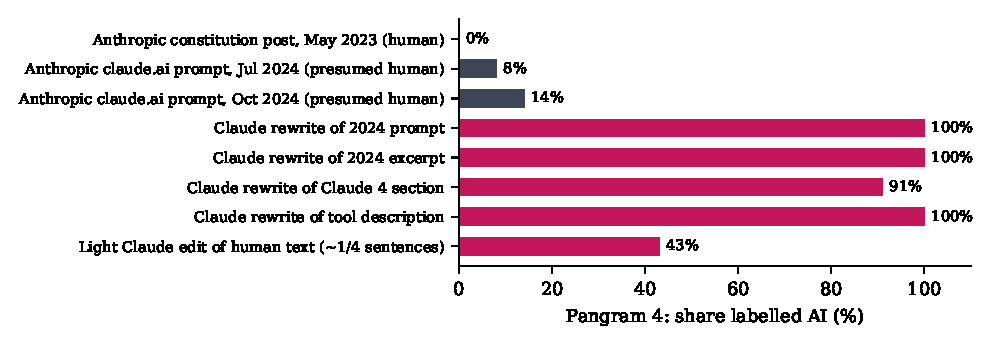
\includegraphics[width=\linewidth]{figs/fig6_controls.pdf}
\caption{Pangram~4 results on controls in the system-prompt genre.}
\label{fig:controls}
\end{figure}

\end{document}
